\section{DeepTune Internal Activation States}
\label{sec:deeptune-internal-states}

In previous sections, DeepTune is shown to automatically outperform state-of-the-art predictive models for which experts have invested a great amount of time in engineering features. This section attempts to illuminate the inner workings, using a single example from Case Study B: predicting the thread coarsening factor for Parboil's \texttt{mriQ} benchmark on four different platforms.

Figure~\ref{fig:viz} shows the DeepTune configuration, with visual overlays showing the internal state. From top to bottom, the input to the model is the 267 lines of OpenCL code for the \texttt{mriQ} kernel. This source code is preprocessed, formatted, and rewritten using variable and function renaming, shown in Figure~\ref{fig:viz}b. The rewritten source code is tokenised and encoded in a $1$-of-$k$ vocabulary. Figure~\ref{fig:viz}c shows the first 80 elements of this encoded sequence as a heat map in which each cell's colour reflects its encoded value. The input, rewriting, and encoding is the same for each of the four platforms.

\begin{figure*}
  \centering %
  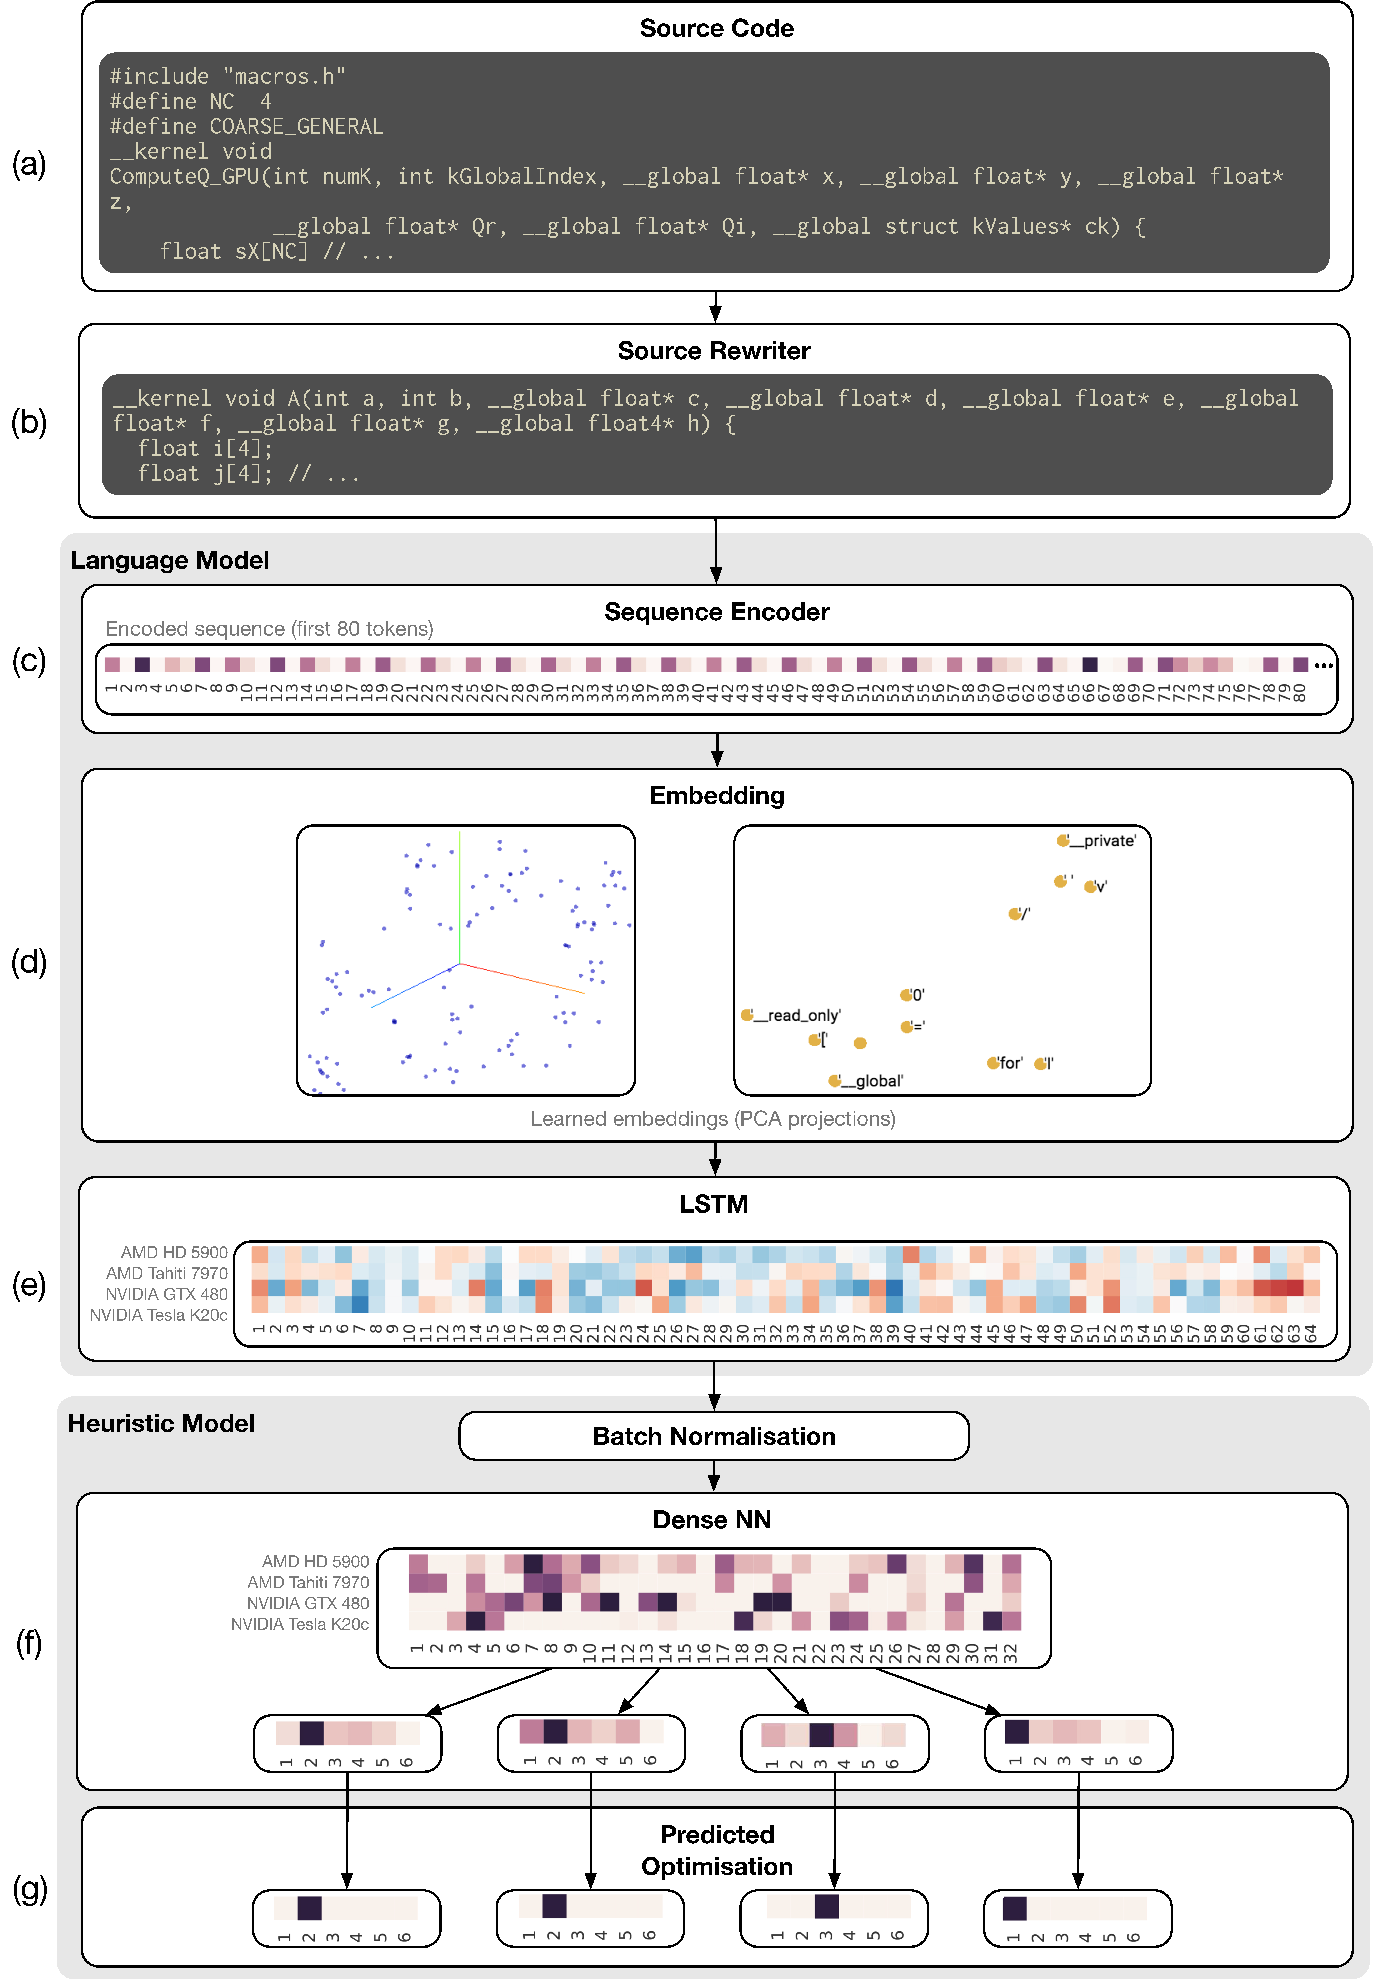
\includegraphics[width=\textwidth]{img/viz}%
    \vspace{-1em}
  \caption{%
    Visualizing the internal state of DeepTune when predicting coarsening factor
    for Parboil's \texttt{mriQ} benchmark on four different architectures. The
    activations in each layer of the four models increasingly diverge the lower
    down the network.%
  }
  \label{fig:viz} %
\end{figure*}


The encoded sequences are then passed into the Embedding layer. This maps each token of the vocabulary to a point in a 64 dimension vector space. Embeddings are learned during training so as to cluster semantically related tokens together. As such, they may differ between the four platforms. Figure~\ref{fig:viz}d shows a PCA projection of the embedding space for one of the platforms, showing multiple clusters of tokens. By honing in on one of the clusters and annotating each point with its corresponding token, it can be observed that the cluster contains the semantically related OpenCL address space modifiers \texttt{\_\_private}, \texttt{\_\_global}, and \texttt{\_\_read\_only}.

Two layers of 64 LSTM neurons model the sequence of embeddings, with the neuron activations of the second layer being used to characterise the entire sequence. Figure~\ref{fig:viz}e shows the neurons in this layer for each of the four platforms, using a red-blue heat map to visualise the intensity of each activation. Comparing the activations between the four platforms, we note a number of neurons in the layer with different responses across platforms. This indicates that the language model is partly specialised to the target platform. Subsequent work~\cite{Ben-nun2018} supports this reasoning, in which performance is slightly degraded by training parts of the language model in a platform-agnostic manner.

As information flows through the network, the layers become progressively more specialised to the specific platform. This can be seen in Figure~\ref{fig:viz}f, which shows the two layers of the heuristic model. The activations within these increasingly diverge. The mean variance of activations across platforms increases threefold compared to the language model, from 0.039 to 0.107. Even the activations of the AMD HD 5900 and AMD Tahiti 7970 platforms are dissimilar, despite the final predicted coarsening factor for both platforms being the same. The largest activation of the output layer is taken in Figure~\ref{fig:viz}g as the final predicted coarsening factor. For this particular program, a state-of-the-art model achieves 54\% of the maximum performance. DeepTune achieves 99\%.
